% ===========================================================
% Chapter 15: Reasoning, Tool Use, and Reinforcement Finetuning
% Part IV: Frontiers
% ===========================================================

\chapter[Reasoning and Reinforcement Finetuning]{Reasoning, Tool Use, and Reinforcement Finetuning}
\label{ch:reasoning}

\begin{quote}
\itshape
If intelligence is a cake, the bulk of the cake is unsupervised learning,
the icing on the cake is supervised learning, and the cherry on the cake
is reinforcement learning.
\par\medskip
\upshape\raggedleft
---\,Yann LeCun, NeurIPS 2016
\end{quote}

\bigskip

For most of the history recounted in this book, reinforcement learning
occupied a curious position in the language-model training pipeline:
theoretically central, practically marginal. The reward signal that
drove RLHF\index{RLHF} (Chapter~\ref{ch:practical-rlhf}) was itself a
learned neural network,\,---\,an imperfect proxy for an
imperfectly-understood goal,\,---\,and every practitioner knew that pushing the
policy too far against such a reward model would lead to reward
hacking rather than genuine improvement. The result was a careful,
tightly KL-constrained training regime in which RL contributed polish
rather than power.

That picture changed sharply between 2024 and 2025. The catalyst was
the recognition that certain domains admit \emph{verifiable} rewards: a
mathematical answer is either correct or incorrect; a piece of code
either passes the test suite or it does not. When rewards can be
computed by a deterministic checking function rather than inferred from
a neural preference model, the dangers of reward hacking evaporate,
and it becomes safe to train with far more aggressive RL for far longer.
The result\,---\,\emph{Reinforcement Learning with Verifiable
Rewards} (RLVR)\index{RLVR}\,---\,produced a qualitative leap in
reasoning ability: models that now spend thousands of tokens thinking
before answering a hard question, that can write and debug complex
programs, and that achieve expert-level performance on competition
mathematics.

This chapter is organised to build understanding progressively. We begin
by making the RLVR objective precise and contrasting it with
the RLHF objective of Part~III
(Section~\ref{sec:rlvr}). We then examine chain-of-thought\index{chain-of-thought}
reasoning as both a prompting technique and a trainable
behavior (Section~\ref{sec:cot}). Section~\ref{sec:training-reasoning}
studies the training recipes used in practice, with DeepSeek R1 as a
worked case study. Section~\ref{sec:inference-scaling} formalises
inference-time scaling: the remarkable phenomenon that generating more
tokens at test time translates into measurable accuracy gains.
Sections~\ref{sec:tool-use} and~\ref{sec:agentic-rl} extend the
framework to \emph{tool use}\index{tool use} and \emph{agentic
RL}\index{agentic RL}, where the model must interact with
external environments over multiple steps. Section~\ref{sec:practical-reasoning}
surveys practical algorithm and infrastructure choices, and
Section~\ref{sec:reasoning-summary} closes with open questions.

% ===========================================================
\section{From RLHF to Reinforcement Learning with Verifiable Rewards}
\label{sec:rlvr}
% ===========================================================

\subsection{The Verification Insight}

Recall from Chapter~\ref{ch:practical-rlhf} that RLHF maximises
\begin{equation}
\label{eq:rlhf-objective}
J_{\mathrm{RLHF}}(\theta)
  = \E_{\pi_\theta}\bigl[r_\phi(x, y)\bigr]
  - \beta\,\KL{\pi_\theta}{\pi_{\mathrm{ref}}},
\end{equation}
where $r_\phi$ is a \emph{learned} reward model trained on human
preference pairs and $\beta > 0$ is a KL penalty coefficient that
prevents the policy from straying too far from a reference model.
The learned reward model introduces two compounding problems. First, it
is an approximation: even a well-trained reward model will assign
incorrect scores to some fraction of responses, and a sufficiently
strong policy can discover and exploit these errors\,---\,a phenomenon
called \emph{reward overoptimisation}\index{reward overoptimisation}
or Goodhart's Law in RL (Chapter~\ref{ch:reward-models}). Second,
training a reward model requires expensive human annotation of
preference pairs, and the resulting model inherits all the biases and
inconsistencies of those annotations.

\index{RLVR!definition}
\emph{Reinforcement Learning with Verifiable Rewards} (RLVR) sidesteps
both problems by replacing the learned reward model with a deterministic
\textbf{verification function}\index{verification function}:
\begin{equation}
\label{eq:rlvr-reward}
r(x, y) = \begin{cases}
  1 & \text{if } \textsc{Verify}(x, y) = \textsc{True}, \\
  0 & \text{otherwise.}
\end{cases}
\end{equation}
The function $\textsc{Verify}$ is domain-specific and entirely
symbolic: for mathematics it extracts the final answer from the
model's response (using a regular expression to locate content in
\texttt{\textbackslash boxed\{\}} notation or after a delimiter such
as \texttt{The answer is:}) and compares it to the ground-truth
solution; for code it executes the response against a test suite and
returns \textsc{True} if all assertions pass.

\begin{definition}[RLVR objective]
\label{def:rlvr}
\index{RLVR!objective}
Let $\mathcal{D}$ be a dataset of (prompt, ground-truth answer) pairs
$(x, a^*)$. The RLVR objective is
\begin{equation}
\label{eq:rlvr-objective}
J_{\mathrm{RLVR}}(\theta)
  = \E_{(x,a^*)\sim\mathcal{D},\,y\sim\pi_\theta(\cdot|x)}
    \bigl[\ind\{\textsc{Verify}(y, a^*)\}\bigr]
  - \beta\,\KL{\pi_\theta}{\pi_{\mathrm{ref}}},
\end{equation}
where $\ind\{\cdot\}$ is the indicator function and the KL term may
be reduced or removed entirely (see Section~\ref{sec:training-reasoning}).
\end{definition}

Because $r$ takes values in $\{0, 1\}$ and is computed by a
deterministic symbolic function, it cannot be over-optimised in the
same way as a neural reward model. A model that learns to produce
correct answers \emph{is} genuinely better; there is no proxy gap to
exploit.

\subsection{Verifiable Domains}
\label{subsec:verifiable-domains}

The power of RLVR depends on having a rich, varied supply of problems
with efficiently verifiable answers. Three domains currently dominate.

\begin{description}[leftmargin=!,labelwidth=3.5cm]
\item[Mathematics] Competition problems drawn from datasets such as
  MATH and AIME admit unique numerical or symbolic answers that can
  be checked exactly. The model is prompted to enclose its final
  answer in a \texttt{\textbackslash boxed\{\}} environment, which a
  regular expression extracts and compares to the ground truth.

\item[Code generation] Problems from LeetCode, HumanEval, or MBPP
  come with unit tests. A model's solution is executed in a sandbox,
  and the reward is $1$ if all tests pass (or a fraction equal to the
  proportion of passing tests for partial-credit variants).

\item[Science and logic] Formal theorem proving (e.g., in Lean 4) and
  structured scientific question-answering with unique factual answers
  are natural extensions. Any domain where a checking function can be
  written is in principle amenable to RLVR.
\end{description}

\subsection{Formal Comparison with the RLHF Objective}
\label{subsec:rlvr-vs-rlhf}

Table~\ref{tab:rlhf-vs-rlvr} contrasts the two frameworks along the
dimensions most relevant to practitioners.

\begin{table}[ht]
\centering
\small
\caption{RLHF versus RLVR: a formal comparison.}
\label{tab:rlhf-vs-rlvr}
\begin{tabular}{@{}lcc@{}}
\toprule
\textbf{Property} & \textbf{RLHF} & \textbf{RLVR} \\
\midrule
Reward source & Learned neural $r_\phi$ & Symbolic $\textsc{Verify}$ \\
Reward range & $\R$ (continuous) & $\{0, 1\}$ (binary) \\
Human annotation & Required for $r_\phi$ & Required for $(x, a^*)$ pairs \\
Over-optimisation risk & High & Negligible \\
KL penalty necessity & Critical & Optional \\
Applicable domains & General & Verifiable domains \\
Reward model cost & $O(\text{response length})$ & $O(\text{checking function})$ \\
\bottomrule
\end{tabular}
\end{table}

The key structural difference is that RLVR converts the RL problem into
one where the reward is \emph{not} a neural network with gradients of
its own, but a read-only oracle. This makes the optimisation landscape
cleaner: there is no inner loop of reward model training to interleave
with policy updates, no distributional shift problem for the reward
model, and no danger of the policy ``finding the gaps'' in a learned
approximation.

\begin{figure}[ht]
\centering
\begin{tikzpicture}[
  node distance=1.8cm and 2.2cm,
  box/.style={rectangle, rounded corners=4pt, draw, thick,
              minimum width=2.4cm, minimum height=0.9cm,
              font=\small, align=center},
  verify/.style={diamond, draw, thick, aspect=2,
                 font=\small\itshape, align=center,
                 inner sep=2pt},
  arrow/.style={-{Stealth[length=7pt]}, thick},
  darrow/.style={{Stealth[length=7pt]}-{Stealth[length=7pt]}, thick, dashed}
]
% Nodes
\node[box, fill=blue!10]  (prompt)    {Prompt $x$};
\node[box, fill=green!10, right=of prompt]  (generate)  {Generate\\$y \sim \pi_\theta(\cdot|x)$};
\node[verify, fill=orange!15, right=of generate] (verify) {Verify\\$(y, a^*)$};
\node[box, fill=red!10, below=1.4cm of verify]   (reward)   {Reward\\$r \in \{0,1\}$};
\node[box, fill=purple!10, left=2.8cm of reward] (update)   {Policy Update\\$\nabla_\theta J_{\mathrm{RLVR}}$};

% Arrows
\draw[arrow] (prompt)   -- (generate);
\draw[arrow] (generate) -- (verify);
\draw[arrow] (verify)   -- node[right]{\small yes/no} (reward);
\draw[arrow] (reward)   -- (update);
\draw[arrow] (update)   -- ++(0,2.3) -| (prompt)
    node[midway, above]{\small repeat over $\mathcal{D}$};

% Ground truth label
\node[box, fill=gray!10, above=1.2cm of verify] (gt) {Ground truth $a^*$};
\draw[arrow, dashed] (gt) -- (verify);
\end{tikzpicture}
\caption{The RLVR training loop. A prompt $x$ from the dataset is fed
  to the current policy $\pi_\theta$, which generates a response $y$.
  A deterministic verification function compares $y$ against the
  ground-truth answer $a^*$ and returns a binary reward. Policy
  gradients are then computed and the cycle repeats. No learned reward
  model is needed.}
\label{fig:rlvr-loop}
\end{figure}

% ===========================================================
\section{Chain-of-Thought Reasoning}
\label{sec:cot}
% ===========================================================

\subsection{The Basic Idea}

Standard autoregressive generation maps a prompt $x$ directly to a
response $y$. Chain-of-thought\index{chain-of-thought} (CoT) generation
interposes a \emph{reasoning trace}\index{reasoning trace} $z$ between
the prompt and the final answer:
\[
x \;\longrightarrow\; z \;\longrightarrow\; a,
\]
where $z$ is a sequence of intermediate reasoning steps and $a$ is the
final answer extracted from the end of the generation. The full
generation $y = (z, a)$ is produced by the same autoregressive model;
$z$ is simply not shown to the user in many deployments.

\begin{example}[Chain-of-thought on a competition problem]
\label{ex:cot-math}
Consider the prompt: \emph{``Find all integer solutions to
$x^2 - 5x + 6 = 0$.''} Without chain-of-thought, a model might emit
the correct answer $\{2, 3\}$ directly (if it has memorised it) or
fail silently. With chain-of-thought, the generation looks like:

\begin{quote}
\texttt{<thinking>}\\
\texttt{I need to factorise $x^2 - 5x + 6$. I am looking for two numbers}\\
\texttt{that multiply to $6$ and add to $-5$. Those numbers are $-2$ and $-3$.}\\
\texttt{So $x^2 - 5x + 6 = (x-2)(x-3)$. Setting each factor to zero:}\\
\texttt{$x - 2 = 0 \Rightarrow x = 2$; $x - 3 = 0 \Rightarrow x = 3$.}\\
\texttt{</thinking>}\\
\texttt{The integer solutions are $x = 2$ and $x = 3$, i.e., $\boxed{2, 3}$.}
\end{quote}

The thinking tokens are invisible to downstream users but are used
during training: the verification function extracts the content of the
\texttt{\textbackslash boxed\{\}} environment to compute the reward.
\end{example}

\subsection{Why Longer Reasoning Helps}
\label{subsec:why-cot-helps}

Chain-of-thought succeeds for an information-theoretic reason.
The probability that a model produces the correct final answer $a^*$
given prompt $x$ can be written, by the chain rule of probability, as
\begin{equation}
\label{eq:cot-chain-rule}
\Prob(a^* \mid x)
  = \sum_{z} \Prob(a^* \mid x, z)\,\Prob(z \mid x).
\end{equation}
Marginalising over intermediate reasoning traces $z$ is equivalent to
using them as a latent variable. A model that can generate a wide
diversity of high-quality reasoning traces effectively performs an
implicit search over solution paths before committing to an answer.
The longer and more varied the reasoning, the finer the implicit
search grid.

This connection to \emph{search}\index{inference-time search} is not merely
metaphorical. We can formalise it by defining the quality of a
reasoning trace $z$ for prompt $x$ and answer $a^*$ as
\[
q(z; x, a^*) = \Prob(a^* \mid x, z).
\]
The model's effective accuracy is $\E_z[q(z; x, a^*)]$, where
the expectation is over the model's distribution over traces. A longer
context window admits more information in $z$, which raises the
ceiling of $q(z; x, a^*)$ for hard problems. Empirically, across
competition mathematics benchmarks, the correlation between average
output token count and accuracy is strong and monotone over several
orders of magnitude of compute\,---\,a scaling law at inference time
(Section~\ref{sec:inference-scaling}).

\subsection{Thinking Tokens and Format}
\label{subsec:thinking-tokens}

Modern reasoning models formalise chain-of-thought by using special
\emph{thinking tokens}\index{thinking tokens}. The generation is
structured as:
\begin{equation}
\label{eq:thinking-format}
y = \underbrace{\texttt{<thinking>}\; z_1 z_2 \cdots z_T
                \;\texttt{</thinking>}}_{\text{reasoning trace, not shown to user}}
    \;\;\underbrace{a_1 a_2 \cdots a_K}_{\text{final answer}}.
\end{equation}
The token sequence $z_1, \ldots, z_T$ is sometimes called the
\emph{scratchpad}\index{scratchpad}. For a simple arithmetic
question, $T$ might be a few dozen tokens; for a hard competition
problem, $T$ may reach tens of thousands of tokens, corresponding to
several minutes of generation on modern hardware.

\begin{remark}[Long context as a prerequisite]
Training reasoning models requires the policy to generate and attend
over very long sequences. The practical enabler of this shift was the
development of efficient attention mechanisms (e.g., FlashAttention)
and context windows of $128\text{k}$--$1\text{M}$ tokens. Without these
engineering advances, the training regime described in
Section~\ref{sec:training-reasoning} would not have been computationally
feasible.
\end{remark}

\subsection{Connection to Inference-Time Compute}
\label{subsec:cot-inference-compute}

The extended generation format of~\eqref{eq:thinking-format}
directly links training to inference-time compute allocation. Define
the \emph{token budget}\index{token budget} $B$ as the maximum number
of tokens the model may generate before producing a final answer. For
a fixed policy $\pi_\theta$, accuracy on a problem set is a
non-decreasing function of $B$:
\[
\text{Acc}(B) = \Prob_{y \sim \pi_\theta(\cdot|x),\,|y| \le B}
               \bigl[\textsc{Verify}(y, a^*) = \textsc{True}\bigr].
\]
Training with RLVR on unconstrained generation teaches the model to
\emph{self-allocate} the token budget: hard problems trigger longer
traces, easy ones resolve quickly. This adaptive allocation is a
key practical advantage over fixed-compute alternatives.

% ===========================================================
\section{Training Reasoning Models}
\label{sec:training-reasoning}
% ===========================================================

\subsection{The Two-Stage Recipe}

The dominant training recipe for reasoning models consists of two
stages, illustrated here using DeepSeek R1 as the canonical open
example.

\begin{description}[leftmargin=!,labelwidth=3.5cm]
\item[Stage~1: SFT cold start] The base pretrained model is first
  fine-tuned with supervised learning on a relatively small dataset of
  high-quality chain-of-thought demonstrations. This stage teaches the
  model the basic format\,---\,the use of \texttt{<thinking>} tags,
  the organisation of multi-step reasoning,\,---\,and ensures that
  subsequent RL has a well-behaved starting distribution to perturb.
  Without this cold start, RLVR training from a base model can diverge
  or produce garbled reasoning traces.

\item[Stage~2: Large-scale RLVR] The SFT-initialised model is then
  trained with a policy-gradient algorithm (typically GRPO or a
  variant; see Section~\ref{sec:practical-reasoning}) over a large
  dataset of verifiable problems. Unlike RLHF, which typically runs
  for $O(1)$ epochs over preference data, RLVR revisits the same
  training problems hundreds or thousands of times, allowing the
  policy to discover and reinforce correct reasoning patterns that were
  only latent in the base model.
\end{description}

\begin{example}[DeepSeek R1 training recipe]
\label{ex:deepseek-r1}
\index{DeepSeek R1}
DeepSeek R1~(January 2025) trained a base model with approximately
600 billion parameters on a curriculum that mixed mathematical
reasoning problems (primarily from competition mathematics datasets),
code synthesis problems with unit-test verification, and general
instruction-following tasks. The RL stage used GRPO with binary
rewards from the verification function, combined with small auxiliary
format rewards to encourage consistent use of the \texttt{<thinking>}
structure. The model was subsequently distilled to smaller sizes
(7B--70B) by fine-tuning on outputs of the full model, making
strong reasoning capabilities accessible on consumer hardware.
\end{example}

\subsection{Difficulty Filtering}
\label{subsec:difficulty-filtering}

A subtle but critical aspect of RLVR training is the choice of which
problems to include in the training set. Recall the policy gradient
update: the gradient of $J_{\mathrm{RLVR}}$ with respect to $\theta$
is non-zero only when different rollouts to the same prompt receive
different rewards. If the current policy solves a problem 100\% of the
time, all rollouts receive reward~$1$, the advantage is identically
zero, and the gradient vanishes. Similarly, if the policy fails 100\%
of the time, all rollouts receive reward~$0$ and no gradient is
generated.\index{difficulty filtering}

\begin{definition}[Problem solvability rate]
\label{def:solvability}
For a problem $x$ with ground truth $a^*$ and policy $\pi_\theta$,
the \textbf{solvability rate} is
\[
\sigma(x) = \Prob_{y \sim \pi_\theta(\cdot|x)}
            \bigl[\textsc{Verify}(y, a^*) = \textsc{True}\bigr],
\]
estimated by sampling $N$ independent rollouts (typically $N = 16$).
\end{definition}

Empirically, problems with $\sigma(x) \in [0.2, 0.8]$ yield the
strongest gradients. Problems outside this window\,---\,too easy or
too hard\,---\,are filtered out of the training set before RLVR
begins. This \emph{offline difficulty filtering} is now a standard
step in reasoning-model pipelines, used by DeepSeek R1, Phi-4
Reasoning, INTELLECT-2, Skywork OR-1, and others.

\subsection{Removing the KL Penalty}
\label{subsec:no-kl}

Standard RLHF uses the KL penalty of~\eqref{eq:rlhf-objective} to
prevent the policy from collapsing onto reward-hacking outputs. In
RLVR, the binary reward cannot be hacked by parroting a fixed output,
because the verification function is deterministic and problem-specific.
As a result, many RLVR practitioners reduce $\beta$ to zero, removing
the KL constraint entirely. This allows the policy to explore more
freely and to discover reasoning patterns that were not present in
the reference model at all. Models that have removed the KL penalty
include Magistral (Mistral, 2025), OpenReasoner-Zero, and Skywork OR-1.

\begin{remark}[KL removal and distributional shift]
Removing the KL penalty does introduce a risk: the policy may drift
to a distribution on which the verifier itself is unreliable (e.g.,
if the model learns to extract answers from positions that the regex
does not match). Careful prompt engineering and verifier robustness
testing are therefore more important in no-KL regimes than in
standard RLHF.
\end{remark}

\subsection{Format Rewards and Length Penalties}
\label{subsec:format-rewards}

In addition to the binary task reward, practitioners commonly add
small auxiliary rewards:

\begin{itemize}[leftmargin=*]
\item \textbf{Format rewards}: A small positive reward ($\approx 0.1$)
  is given when the response correctly uses the \texttt{<thinking>}
  \ldots\ \texttt{</thinking>} structure before producing the final
  answer. This prevents the model from drifting to a format that is
  difficult to parse.

\item \textbf{Length penalties}: Reasoning traces that are longer than
  necessary consume extra inference compute without improving accuracy.
  A penalty proportional to $\max(0, |z| - L_{\max})$ discourages
  pathological overthinking\index{overthinking} while preserving the
  model's ability to use long traces when genuinely needed. Some
  recipes (e.g., Kimi 1.5) use a progressive length curriculum:
  the model first learns to reason within a tight token budget and
  the budget is expanded as training progresses.

\item \textbf{Language consistency rewards}: Multilingual models can
  drift to switching languages mid-trace (e.g., starting in English
  and finishing in Chinese), which degrades user experience. A binary
  reward for language consistency is used by DeepSeek R1 and Magistral.
\end{itemize}

\subsection{Loss Normalisation and the GRPO Bias}
\label{subsec:loss-norm}

The GRPO algorithm (Chapter~\ref{ch:pg}) computes advantages by
normalising rewards within each group of rollouts for the same
prompt. A subtle consequence is that the contribution of a problem
to the total loss is independent of the number of rollouts generated
for it. If harder problems systematically require more tokens,
normalising at the group level can over-weight easy, short problems
and under-weight hard ones. Several reasoning model recipes
(including Magistral and MiMo) address this by normalising advantages
at the \emph{batch} level rather than the group level, or by
weighting the loss by token count.

\subsection{Self-Taught Reasoning and Distillation}
\label{subsec:star-distill}

Two important variants of the standard recipe depart from pure RL.

\textbf{STaR}\index{STaR} (Self-Taught Reasoner; Zeiler et al., 2022)
and its descendant \textbf{Quiet-STaR}\index{Quiet-STaR} approximate
the policy gradient by iterating between: (1) sampling reasoning traces
from the current model, (2) filtering to those that lead to correct
answers, and (3) fine-tuning the model on the filtered traces with
cross-entropy loss. This is equivalent to a simplified form of RL where
the reward is binary and the baseline is zero. STaR approximates the
gradient of~\eqref{eq:rlvr-objective} without requiring an explicit
advantage computation, at the cost of some statistical efficiency.
Quiet-STaR adds the innovation of generating thinking tokens before
every token prediction, not just at the beginning of the response,
which provides a richer training signal.

\textbf{Distillation}\index{distillation!reasoning} transfers
reasoning capability from a large, RLVR-trained model to a smaller
student model via supervised fine-tuning on the teacher's
chain-of-thought outputs. Because the student learns from the teacher's
completed reasoning traces\,---\,including the thinking
tokens\,---\,it can reach reasoning performance far above what
direct RLVR on the student alone would achieve. DeepSeek R1 released
distilled checkpoints at 7B and 70B that outperformed their same-size
non-distilled counterparts on competition mathematics.

% ===========================================================
\section{Inference-Time Scaling}
\label{sec:inference-scaling}
% ===========================================================

\subsection{The Test-Time Compute Hypothesis}

Inference-time scaling\index{inference-time scaling} is the
empirical finding that, for a fixed trained policy, allocating more
computation at test time\,---\,by generating more tokens, more
responses, or both\,---\,leads to measurable improvements in task
accuracy. This is distinct from training-time scaling (larger models
or more training data): it is scaling at deployment.

Let $\mathcal{P}$ denote a set of benchmark problems and let
$C$ be the compute budget measured in FLOPs (or, equivalently, in
total output tokens generated). The inference scaling law asserts that
there exists a function $f$ such that
\begin{equation}
\label{eq:inference-scaling}
\text{Acc}(C) \approx f(C) = f_0 + \alpha \log C + O((\log C)^{-1}),
\end{equation}
for constants $f_0$ and $\alpha > 0$. Empirically, this log-linear
relationship holds over two to three orders of magnitude of test-time
compute on competition mathematics benchmarks, before saturating as
problems are exhausted.

\begin{figure}[ht]
\centering
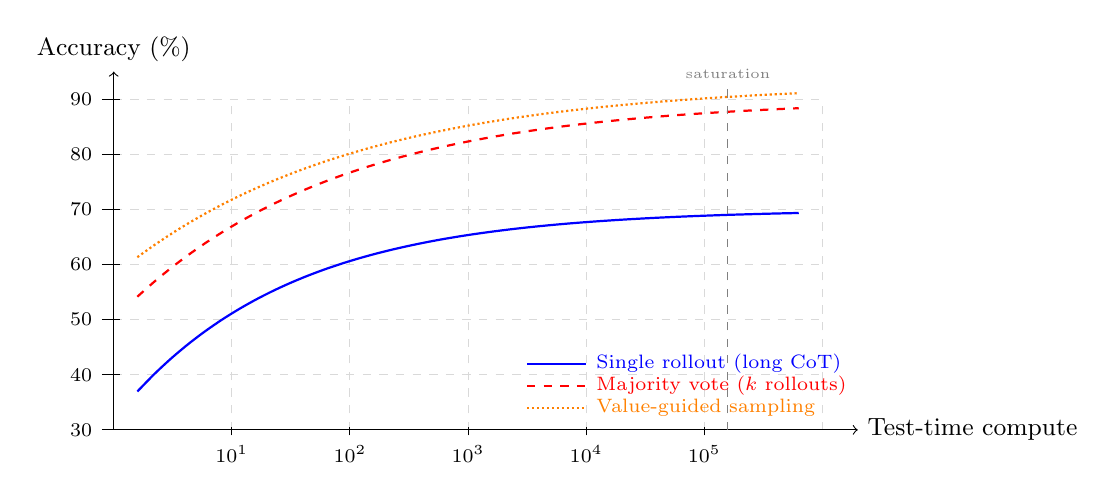
\begin{tikzpicture}[xscale=1.5, yscale=0.07]
  % Grid
  \draw[gray!30, dashed] (0,30) grid[xstep=1,ystep=10] (6,90);
  % Axes
  \draw[->] (0,30) -- (6.3,30) node[right, font=\small]{Test-time compute};
  \draw[->] (0,30) -- (0,95) node[above, font=\small]{Accuracy (\%)};
  % Y ticks
  \foreach \y in {30,40,50,60,70,80,90}
    \draw (-0.1,\y) node[left, font=\scriptsize]{\y} -- (0.05,\y);
  % X ticks
  \foreach \x/\lab in {1/$10^1$,2/$10^2$,3/$10^3$,4/$10^4$,5/$10^5$}
    \draw (\x,29) node[below, font=\scriptsize]{\lab} -- (\x,30.5);
  % Single rollout (blue)
  \draw[thick, blue] plot[smooth, domain=0.2:5.8, samples=40]
    (\x, {32 + 38*(1 - exp(-0.7*\x))});
  % Majority vote (red dashed)
  \draw[thick, red, dashed] plot[smooth, domain=0.2:5.8, samples=40]
    (\x, {50 + 40*(1 - exp(-0.55*\x))});
  % Value-guided (orange dotted)
  \draw[thick, orange, densely dotted] plot[smooth, domain=0.2:5.8, samples=40]
    (\x, {58 + 35*(1 - exp(-0.5*\x))});
  % Saturation line
  \draw[gray, dashed] (5.2,30) -- (5.2,92) node[above, font=\tiny, gray]{saturation};
  % Legend
  \draw[thick, blue] (3.5,42) -- ++(0.5,0) node[right, font=\scriptsize]{Single rollout (long CoT)};
  \draw[thick, red, dashed] (3.5,38) -- ++(0.5,0) node[right, font=\scriptsize]{Majority vote ($k$ rollouts)};
  \draw[thick, orange, densely dotted] (3.5,34) -- ++(0.5,0) node[right, font=\scriptsize]{Value-guided sampling};
\end{tikzpicture}
\caption{Schematic inference-time scaling curves on competition
  mathematics. Accuracy grows log-linearly with test-time compute for
  a range of strategies. Majority voting over $k$ parallel rollouts
  offers higher accuracy at the same compute than a single long
  rollout; value-guided sampling extracts further gains by using a
  process reward model to steer beam search. All curves saturate once
  the model's capability ceiling is reached.}
\label{fig:inference-scaling}
\end{figure}

\subsection{Majority Voting}
\label{subsec:majority-voting}

The simplest inference-time scaling strategy is \emph{majority
voting}\index{majority voting} (also called \emph{self-consistency}):
sample $k$ independent responses $y_1, \ldots, y_k$ from the policy,
extract the final answer $a_i$ from each, and return the plurality
answer:
\begin{equation}
\label{eq:majority-vote}
\hat{a} = \argmax_{a} \sum_{i=1}^{k} \ind\{a_i = a\}.
\end{equation}
If individual responses are correct with probability $p >
\frac{1}{2}$, the majority vote is correct with probability that
approaches~$1$ exponentially fast in $k$ (a consequence of the
law of large numbers). In practice, $k = 8$--$64$ rollouts
suffices for most competition benchmarks.

\begin{proposition}[Majority vote accuracy bound]
\label{prop:majority-vote}
Suppose each of $k$ independent rollouts is correct with probability
$p \in (\frac{1}{2}, 1)$ and there are at most $m$ possible answers.
The majority vote errs with probability at most
\[
\Prob(\hat{a} \ne a^*) \le
\binom{k}{\lfloor k/2 \rfloor} p^{\lfloor k/2 \rfloor}(1-p)^{k - \lfloor k/2 \rfloor}
\;\le\; \exp\bigl(-k\,D_{\mathrm{KL}}(1/2 \,\|\, 1-p)\bigr),
\]
where $D_{\mathrm{KL}}$ denotes the binary KL divergence. The error
decreases exponentially in $k$.
\end{proposition}

\subsection{Value-Guided Sampling}
\label{subsec:value-guided}

Majority voting treats all rollouts as equally plausible. A more
sophisticated strategy uses a \emph{process reward model}
(PRM)\index{process reward model} that assigns scores to
\emph{intermediate} reasoning steps, not only to the final answer.
Given a partial trace $z_{1:t}$, the PRM predicts the probability
that the reasoning will lead to a correct final answer. This score
can guide generation via beam search or best-of-$k$ selection:
\begin{equation}
\label{eq:prm-selection}
\hat{y} = \argmax_{y \in \{y_1,\ldots,y_k\}} \mathrm{PRM}(y).
\end{equation}
Value-guided sampling consistently outperforms majority voting at equal
compute, because it concentrates sampling budget on promising reasoning
paths rather than averaging over all of them. The overhead is the cost
of running the PRM scorer, which is typically a much smaller model
than the policy.

\subsection{Compute-Optimal Inference}
\label{subsec:compute-optimal}

A natural question is how to split a fixed compute budget $C$ between
the length of individual traces (more thinking tokens per rollout)
and the number of rollouts $k$. Defining the per-rollout cost as
$c(B) \propto B$ (where $B$ is the token budget per rollout), the
total compute is $C = k \cdot c(B)$. The compute-optimal strategy
solves:
\[
(k^*, B^*) = \argmax_{k,\,B:\,k\cdot B = C}\; \text{Acc}(k, B),
\]
where $\text{Acc}(k, B)$ is the accuracy under majority vote with $k$
rollouts of length $B$. Empirically, this tradeoff favours longer
individual traces for harder problems (which need deep reasoning) and
more rollouts for easier problems (where the model is already close
to correct and diversity is valuable). Adaptive token-budget allocation
within a single long generation is an active research direction.

% ===========================================================
\section{Tool Use and Function Calling}
\label{sec:tool-use}
% ===========================================================

\subsection{Motivation}

Language models trained purely on text have a fundamental limitation:
they cannot access information beyond their training data, execute
code, or interact with external services. Tool use\index{tool use}
extends the model's action space from token generation to
\emph{function calls}: structured outputs that request the execution
of an external tool and embed the result in the subsequent generation.
This is a qualitative extension of the generation paradigm:
\begin{equation}
\label{eq:tool-loop}
x \;\longrightarrow\; (z_1, \underbrace{f_1(q_1)}_{\text{tool call}},
r_1, z_2, \underbrace{f_2(q_2)}_{\text{tool call}}, r_2, \ldots, a),
\end{equation}
where $f_i$ is a tool (e.g., a web search API or a Python interpreter),
$q_i$ is the query the model submits to it, $r_i$ is the result
returned, and the model's generation interleaves reasoning ($z_i$)
with tool calls and their results.

\subsection{Function Calling Format}
\label{subsec:function-calling-format}

In practice, tool calls are expressed as structured JSON objects
embedded in the generation stream. A typical format:

\begin{example}[Tool call in JSON format]
\label{ex:tool-call-json}
\index{function calling!format}
Consider a model answering: \emph{``What is the current population
of France?''} The generation might look like:

\begin{quote}
\small
\texttt{<thinking>}\\
\texttt{I need to look up the current population of France.}\\
\texttt{</thinking>}\\[0.3em]
\texttt{\{}\\\
\texttt{\ \ "tool": "web\_search",}\\
\texttt{\ \ "query": "current population of France 2025"}\\
\texttt{\}}\\[0.3em]
\textit{[Tool result injected: ``France population: approximately 68.4 million (2025)'']}\\[0.3em]
\texttt{The current population of France is approximately 68.4 million.}
\end{quote}

The JSON object is parsed by the inference runtime, the tool is
invoked, and the result is appended to the model's context before
generation continues. The model never sees raw API internals; it
interacts with a clean interface of named tools with typed parameters.
\end{example}

The model must learn three capabilities simultaneously: (1) to
recognise when a tool call is needed, (2) to emit well-formed JSON
that matches the tool's schema, and (3) to correctly incorporate the
tool's result into its subsequent reasoning.

\subsection{Training Tool Use}
\label{subsec:training-tool-use}

Tool use is typically trained in two stages:

\begin{description}[leftmargin=!,labelwidth=3.5cm]
\item[SFT on demonstrations] The model is first fine-tuned on a
  curated dataset of tool-use trajectories: (prompt, tool-call
  sequence, final answer) triples collected from human demonstrations
  or from larger models. This teaches the model the format and the
  basic decision of when to call a tool.

\item[RL for multi-step tool use] SFT alone is insufficient for
  complex, multi-step tool-use scenarios, because the correct sequence
  of tool calls depends on the results of previous calls in a way that
  is difficult to enumerate in a fixed demonstration dataset. RL allows
  the model to discover effective tool-calling strategies by
  interacting with a live tool environment and receiving a binary
  reward for task completion.
\end{description}

The reward signal for tool-use RL is typically outcome-based: the
model receives reward~$1$ if the final answer (after all tool calls)
is correct, and~$0$ otherwise. This is precisely the RLVR framework
of Section~\ref{sec:rlvr}, now extended to multi-step trajectories.
The environment is the tool ecosystem itself.

\subsection{SWiRL: Step-Wise RL for Tool Use}
\label{subsec:swirl}

\index{SWiRL}
\textbf{SWiRL} (Step-Wise Reinforcement Learning) is a framework
designed specifically for multi-step tool-use tasks where outcome
rewards are sparse. Rather than waiting until the end of a trajectory
to assign reward, SWiRL provides \emph{process rewards} at each tool
call. A step reward $r_t$ is computed by a process reward model that
evaluates whether the $t$-th tool call was useful and well-formed.
The total reward is:
\begin{equation}
\label{eq:swirl-reward}
R = \sum_{t=1}^{T} \gamma^{t-1} r_t + \lambda \cdot r_{\mathrm{outcome}},
\end{equation}
where $r_{\mathrm{outcome}} \in \{0, 1\}$ is the binary task-completion
reward and $\lambda$ is a weighting hyperparameter. Step rewards
reduce variance in the policy gradient estimate by providing more
frequent feedback, at the cost of requiring a step-level evaluator.

% ===========================================================
\section{Multi-Step Agents and Agentic RL}
\label{sec:agentic-rl}
% ===========================================================

\subsection{The Agent Loop}

When tool use extends over many steps and the model must plan across
a long horizon, we enter the regime of \emph{agentic RL}\index{agentic RL}.
The model now functions as a full RL agent interacting with an
environment $\mathcal{E}$ (the collection of available tools and
external systems). The standard agent loop is:

\begin{enumerate}
\item \textbf{Observe}: Receive an observation $o_t$ from the
  environment (e.g., the contents of a webpage, the output of a
  terminal command, or the response of an API).
\item \textbf{Think}: Generate a reasoning trace $z_t$ conditioned
  on the full context $(x, o_1, a_1, \ldots, o_{t-1}, a_{t-1}, o_t)$.
\item \textbf{Act}: Emit an action $a_t$, which may be a tool call,
  a navigation command, or a text output.
\item \textbf{Observe}: Receive $o_{t+1}$ from the environment. Go to~2.
\end{enumerate}

This is precisely the MDP agent loop from Chapter~\ref{ch:mdp}, now
instantiated with a language model as the policy and a software
environment as the transition function.

\begin{figure}[ht]
\centering
% Simplified agentic RL loop: clear layout with labels placed away from arrows
\begin{tikzpicture}[
  node distance=1.4cm and 2.6cm,
  box/.style={rectangle, rounded corners=4pt, draw, thick,
              minimum width=2.4cm, minimum height=0.8cm,
              font=\small, align=center},
  grp/.style={rectangle, rounded corners=6pt, draw, thick,
              minimum width=2.8cm, minimum height=2.8cm,
              font=\small, align=center},
  arrow/.style={-{Stealth[length=6pt]}, thick},
  darrow/.style={-{Stealth[length=6pt]}, thick, dashed},
  lbl/.style={font=\scriptsize, fill=white, inner sep=1pt},
]

% ---- Agent group (left column) ----
\node[grp, fill=blue!8] (agentbox) {};
\node[font=\small\bfseries, above=0.05cm of agentbox.north]
      {LLM Agent $\pi_\theta$};
\node[box, fill=blue!18, minimum width=2.0cm, minimum height=0.6cm,
      above=0.05cm of agentbox.center] (think) {Think $z_t$};
\node[box, fill=blue!18, minimum width=2.0cm, minimum height=0.6cm,
      below=0.05cm of agentbox.center] (act) {Act $a_t$};

% ---- Environment group (right column) ----
\node[grp, fill=orange!8, right=2.6cm of agentbox] (envbox) {};
\node[font=\small\bfseries, above=0.05cm of envbox.north]
      {Environment};
\node[box, fill=orange!18, minimum width=2.0cm, minimum height=0.6cm,
      above=0.05cm of envbox.center] (tools) {Tools \& APIs};
\node[box, fill=orange!18, minimum width=2.0cm, minimum height=0.6cm,
      below=0.05cm of envbox.center] (envobs) {Obs.\ $o_{t+1}$};

% ---- Task (above agent) ----
\node[box, fill=green!10, above=1.2cm of agentbox, minimum width=2.6cm]
      (task) {Task / Prompt $x$};

% ---- Context window (below agent) ----
\node[box, fill=gray!12, below=1.2cm of agentbox, minimum width=2.6cm]
      (ctx) {Context window};

% ---- Reward (below environment) ----
\node[box, fill=red!10, below=1.2cm of envbox, minimum width=2.6cm]
      (reward) {Reward $r$};

% ---- Arrows ----
% Task -> Agent
\draw[arrow] (task.south) -- (agentbox.north);

% Act -> Tools (action)
\draw[arrow] ([yshift=-2pt]act.east) -- ([yshift=-2pt]tools.west)
      node[lbl, below, midway] {action $a_t$};

% Obs -> Think (observation, above midline)
\draw[arrow] ([yshift=2pt]envobs.west) -- ([yshift=2pt]think.east)
      node[lbl, above, midway] {obs.\ $o_{t+1}$};

% Agent -> Context
\draw[arrow] (agentbox.south) -- (ctx.north);

% Context -> Reward
\draw[arrow] (ctx.east) -- (reward.west)
      node[lbl, below, midway] {episode end};

% Reward -> Env (dashed, verify outcome)
\draw[darrow] (reward.north) -- (envbox.south)
      node[lbl, right, midway] {verify};

\end{tikzpicture}
\caption{The agentic RL loop. The LLM agent $\pi_\theta$ observes the
  environment, generates a reasoning trace, and emits an action (a
  tool call or text output). The environment executes the action and
  returns an observation. The full context accumulates in the model's
  context window. After the episode terminates, a reward signal
  (outcome-based or step-based) is computed and used for a policy
  gradient update.}
\label{fig:agent-loop}
\end{figure}

\subsection{Agentic Tasks and Environments}
\label{subsec:agentic-tasks}

Agentic RL has been applied to a growing range of tasks:

\begin{description}[leftmargin=!,labelwidth=3.5cm]
\item[Web browsing] The agent navigates a web browser (via Playwright
  or similar), reading pages, clicking links, and filling forms to
  complete information-retrieval or transaction tasks. Reward is
  binary: the task goal is achieved or not.

\item[Code execution] The agent writes code, executes it in a
  sandboxed Python interpreter, reads the output, and iterates. The
  unit-test reward signal from Section~\ref{sec:rlvr} applies
  directly.

\item[API interaction] The agent calls REST APIs, reads responses,
  and chains API calls to complete multi-step workflows (e.g., booking
  a calendar event after looking up availability). Reward comes from
  verifying the final system state.

\item[Repository-level coding] The agent reads and writes files in a
  code repository, runs tests, and resolves issues from bug reports.
  SWE-bench\index{SWE-bench} is the standard benchmark, measuring
  the fraction of GitHub issues resolved by the agent.
\end{description}

\subsection{Credit Assignment in Multi-Step Trajectories}
\label{subsec:credit-agentic}

The fundamental challenge of agentic RL\index{credit assignment!agentic}
is credit assignment: when a trajectory of $T$ steps receives a single
terminal reward, each of the $T$ actions must be credited appropriately.
This is the delayed-reward problem from classical RL
(Chapter~\ref{ch:td}), magnified by the length of language model
trajectories.

Two paradigms address this:

\begin{itemize}[leftmargin=*]
\item \textbf{Outcome rewards}: Credit each token in the trajectory
  with the same terminal reward (possibly discounted). This is simple
  but high-variance: early actions that set up success are rewarded
  equally with the single final token that confirms success.

\item \textbf{Process rewards}: Train a step-level PRM to assign
  rewards $r_t$ at each step. This reduces variance dramatically
  but requires additional supervision to train the PRM. The PRM can
  be trained on human annotations of which intermediate steps are
  correct, or (more scalably) using Monte Carlo rollouts from each
  intermediate state to estimate the probability of eventual success.
\end{itemize}

The tradeoff between process and outcome rewards (discussed more
broadly in Chapter~\ref{ch:reward-models}) is particularly sharp in
the agentic setting, where trajectories may span dozens of tool calls
and hundreds of thousands of tokens.

\subsection{Exploration in Agentic RL}
\label{subsec:agentic-exploration}

Classical RL exploration strategies (epsilon-greedy, Thompson
sampling, intrinsic motivation; Chapter~\ref{ch:intro}) take on new
character when the policy is a language model. The model's prior from
pretraining already encodes a rich distribution over action sequences,
which provides implicit exploration. However, that prior may be
concentrated on safe, familiar action sequences that avoid the
long-horizon strategies needed for hard agentic tasks.

Practical approaches to agentic exploration include:

\begin{itemize}[leftmargin=*]
\item \textbf{Temperature scaling}: Increasing generation temperature
  at training time diversifies rollouts, analogous to increasing
  epsilon in epsilon-greedy.

\item \textbf{Curriculum over task difficulty}: Starting with short,
  easy tasks and progressively introducing longer, harder ones ensures
  the model receives adequate feedback signals throughout training.

\item \textbf{Environment randomisation}: Varying task instances
  (different web pages, different code repositories, different API
  endpoints) prevents the policy from memorising specific trajectories.
\end{itemize}

% ===========================================================
\section{Practical Considerations}
\label{sec:practical-reasoning}
% ===========================================================

\subsection{Algorithm Choices}
\label{subsec:algorithm-choices}

Table~\ref{tab:reasoning-algorithms} summarises the main RL algorithms
used for reasoning and agentic training.

\begin{table}[ht]
\centering
\footnotesize
\caption{Policy optimisation algorithms for reasoning model training.}
\label{tab:reasoning-algorithms}
\begin{tabular}{@{}lp{3.5cm}p{2.5cm}p{2.5cm}@{}}
\toprule
\textbf{Algorithm} & \textbf{Mechanism} & \textbf{Key property}
  & \textbf{Used by} \\
\midrule
PPO & Clipped surr.\ + value net
  & Stable, well-understood & Tülu~3, Phi-4 \\
GRPO & Group-norm.\ advantages, no value net
  & Memory-efficient & DeepSeek R1, Qwen~3 \\
DAPO & Asymmetric clipping
  & Better exploration & RAGEN, INTELLECT-2 \\
CISPO & Clipped importance sampling
  & Off-policy stable & MiniMax-M1 \\
MuonClip & QK-norm clipping
  & Prevents loss spikes & Kimi~K2 \\
\bottomrule
\end{tabular}
\end{table}

\textbf{PPO}\index{PPO!reasoning} (Proximal Policy Optimisation)
remains the most widely studied algorithm for RL fine-tuning, owing
to its theoretical guarantees and extensive empirical track record.
It requires maintaining a separate value network, which doubles the
memory footprint but reduces gradient variance through a learned baseline.

\textbf{GRPO}\index{GRPO} (Group Relative Policy Optimisation) avoids
the value network by computing per-prompt advantage estimates from
the empirical mean and variance of rewards within a group of $k$
rollouts:
\begin{equation}
\label{eq:grpo-advantage}
\hat{A}_i = \frac{r_i - \bar{r}}{\sigma_r}, \qquad
\bar{r} = \frac{1}{k}\sum_{j=1}^k r_j, \quad
\sigma_r = \sqrt{\frac{1}{k}\sum_{j=1}^k (r_j - \bar{r})^2}.
\end{equation}
With binary RLVR rewards, $r_i \in \{0, 1\}$, this simplifies to
$\hat{A}_i = +\sigma_r^{-1}$ for correct completions and
$\hat{A}_i = -\bar{r}/\sigma_r$ for incorrect ones. GRPO has become
dominant in reasoning model training because it is memory-efficient
and easy to implement.

\textbf{DAPO}\index{DAPO} (Decoupled Clip and Dynamic Sampling Policy
Optimisation) modifies GRPO by using asymmetric clipping bounds: a
larger clip on the positive side allows more aggressive updates toward
high-reward responses while the negative-side clip remains conservative.
This promotes exploration of correct reasoning strategies that the
current policy reaches only rarely.

\subsection{Online vs.\ Offline RL}
\label{subsec:online-offline}

\begin{description}[leftmargin=!,labelwidth=3.5cm]
\item[Online RL] Rollouts are generated from the current policy
  $\pi_\theta$ and immediately used for a gradient update. This keeps
  the training distribution on-policy, which is theoretically clean
  but practically slow: the policy must wait for generation to complete
  before updating.

\item[Offline RL] Rollouts are pre-generated (from an earlier
  checkpoint of the policy or from a different model) and stored in a
  replay buffer. Updates use importance weights to correct for the
  distributional mismatch. Offline RL improves throughput dramatically
  but introduces off-policy bias if the replay buffer is stale.

\item[Asynchronous RL] A practical compromise used by several
  reasoning model recipes: generation runs asynchronously on one set
  of GPUs while gradient updates proceed on another. This keeps the
  policy nearly on-policy while avoiding idle compute.
\end{description}

\subsection{Infrastructure at Scale}
\label{subsec:infra}

Training a reasoning model requires infrastructure that differs from
standard language model pre-training in several ways:

\begin{itemize}[leftmargin=*]
\item \textbf{Generation throughput}: RLVR training requires sampling
  $k = 8$--$16$ rollouts per prompt, each potentially thousands of
  tokens long. Efficient batched generation with continuous batching
  (as in vLLM) is essential.

\item \textbf{Verification at scale}: The verifier (regex extractor,
  code sandbox) must run in parallel for thousands of completions per
  second without becoming the bottleneck. Code verification is
  particularly expensive because it requires process isolation.

\item \textbf{Memory management}: GRPO's elimination of the value
  network halves GPU memory consumption relative to PPO, but storing
  $k$ full rollout sequences per prompt still requires careful memory
  planning.

\item \textbf{Reward normalisation and logging}: Because RLVR rewards
  are binary and sparse early in training, careful monitoring of the
  moving-average reward, rollout length, and format-reward compliance
  is necessary to detect training instabilities before they cascade.
\end{itemize}

\subsection{Open-Source Tooling}
\label{subsec:open-source-tooling}

Several open-source frameworks have made RLVR training accessible
beyond well-resourced industrial labs:

\begin{description}[leftmargin=!,labelwidth=2.5cm]
\item[TRL] Hugging Face's Transformer Reinforcement Learning library
  implements PPO, GRPO, and DPO with first-class support for
  verifiable rewards. Its \texttt{GRPOTrainer} integrates directly
  with the \texttt{datasets} and \texttt{transformers} ecosystems.

\item[veRL] A high-throughput RL training framework from Volcengine
  that supports asynchronous generation--update pipelines and
  achieves state-of-the-art training throughput for large models.

\item[OpenRLHF] A distributed RLHF and RLVR framework built on
  DeepSpeed and Ray, supporting models up to hundreds of billions of
  parameters with flexible reward function APIs.
\end{description}

% ===========================================================
\section{Summary and Open Questions}
\label{sec:reasoning-summary}
% ===========================================================

This chapter has traced the arc from RLHF\,---\,where a learned
reward model provided imperfect preference signals\,---\,to RLVR,
where deterministic verification functions enable aggressive,
long-horizon RL training on verifiable domains. The key conceptual
contributions are:

\begin{itemize}[leftmargin=*]
\item \textbf{Verifiable rewards} eliminate the reward model as a
  bottleneck and a failure mode. Binary rewards from checking functions
  are noise-free and cannot be over-optimised.

\item \textbf{Chain-of-thought reasoning} connects token generation
  to implicit search: longer reasoning traces implement a finer
  search over solution paths.

\item \textbf{Inference-time scaling} shows that compute can be
  productively spent at deployment, not only at training. Majority
  voting and value-guided sampling extract accuracy gains from
  additional generation without retraining.

\item \textbf{Tool use and agentic RL} extend the framework to
  interactive environments, transforming language models from passive
  text generators into active problem-solving agents.
\end{itemize}

\paragraph{Open questions.} The field is moving rapidly, and several
fundamental questions remain unresolved:

\begin{itemize}[leftmargin=*]
\item \textbf{Generalisation of RLVR}: Do reasoning skills learned
  on mathematics and code transfer to unverifiable domains
  (open-ended writing, strategic reasoning, safety)? Early evidence
  suggests partial transfer, but the mechanism is unclear.

\item \textbf{Scaling limits}: How far do inference-time scaling laws
  extend? At what point does generating more tokens yield diminishing
  returns independent of model capacity?

\item \textbf{Process reward models at scale}: Training a reliable
  PRM requires step-level supervision, which is expensive to collect.
  Monte Carlo estimation of step correctness is noisy. Better methods
  for PRM training are an active research area.

\item \textbf{Safety of agentic systems}: An agent that can browse
  the web, execute code, and call APIs has a vastly larger action
  space than a text-only chatbot. Aligning the objectives of
  multi-step agents with human values is an open challenge that
  classical RLHF was not designed to address.

\item \textbf{Interplay with pretraining}: Several results suggest
  that a certain level of pretraining capability is a prerequisite
  for RLVR to work. Understanding the threshold and how to lower it
  would democratise reasoning training.
\end{itemize}

% ===========================================================
\section*{Exercises}
\addcontentsline{toc}{section}{Exercises}
% ===========================================================

\begin{exercise}
\label{ex:rlvr-gradient}
Consider the RLVR objective in~\eqref{eq:rlvr-objective} with $\beta = 0$.
Show that the policy gradient of $J_{\mathrm{RLVR}}(\theta)$ with
respect to $\theta$ can be written as
\[
\nabla_\theta J_{\mathrm{RLVR}}(\theta)
  = \E_{x, y}\bigl[\ind\{\textsc{Verify}(y, a^*)\}\,
    \nabla_\theta \log \pi_\theta(y \mid x)\bigr],
\]
starting from first principles using the log-derivative trick. How
does this reduce to the REINFORCE\index{REINFORCE} gradient of
Chapter~\ref{ch:pg} with $r(y) = \ind\{\textsc{Verify}(y,a^*)\}$?
\end{exercise}

\begin{exercise}
\label{ex:majority-vote-bound}
Prove Proposition~\ref{prop:majority-vote}. Specifically, show that
for $k$ independent Bernoulli($p$) trials with $p > 1/2$, the
probability that fewer than $k/2$ successes occur is bounded above
by $\exp(-k\,D_{\mathrm{KL}}(1/2\,\|\,1-p))$ using Hoeffding's inequality
or Chernoff bounds.
\end{exercise}

\begin{exercise}
\label{ex:grpo-advantage}
Suppose $k = 4$ rollouts for a prompt receive rewards $r = (1, 1, 0, 0)$.
Compute the GRPO advantage estimates $\hat{A}_i$ from~\eqref{eq:grpo-advantage}.
Now suppose instead $r = (1, 0, 0, 0)$. Compute $\hat{A}_i$ again.
Compare the magnitude of the gradient signal in the two cases and
explain why the second scenario gives stronger feedback to the correct
rollout even though there is only one correct rollout.
\end{exercise}

\begin{exercise}
\label{ex:difficulty-filter}
A training dataset contains 10{,}000 problems. You sample $N = 16$
rollouts per problem and find that 2{,}000 problems have solvability
rate $\sigma < 0.2$, 5{,}000 have $\sigma \in [0.2, 0.8]$, and 3{,}000
have $\sigma > 0.8$.
\begin{enumerate}[label=(\alph*)]
\item What fraction of compute is ``wasted'' on uninformative problems
  (those with $\sigma < 0.2$ or $\sigma > 0.8$)?
\item How does difficulty filtering change the effective dataset
  size available for gradient updates?
\item Propose a dynamic difficulty curriculum that avoids discarding
  hard problems permanently.
\end{enumerate}
\end{exercise}

\begin{exercise}
\label{ex:cot-information}
Using the decomposition~\eqref{eq:cot-chain-rule}, argue informally
why (a) chain-of-thought improves accuracy for hard multi-step
problems but (b) is largely redundant for problems that the model can
answer correctly in a single step. What does this imply for the
desiderata of a \emph{toggleable} reasoning mode?
\end{exercise}

\begin{exercise}
\label{ex:tool-calling-reward}
A model is solving the following task via tool use: retrieve the
population of France and the population of Germany, then output their
ratio. Write a Python function \texttt{verify(trajectory)} that takes
a list of (action, observation) pairs and returns a reward in
$\{0, 1\}$. Your function should handle: (a) the model calling tools
in the wrong order, (b) the model failing to call a required tool,
and (c) arithmetic errors in the final computation.
\end{exercise}

\begin{exercise}
\label{ex:process-vs-outcome}
Consider a multi-step agent completing a 5-step task. The outcome
reward is $+1$ only on task completion. Suppose the agent succeeds on
the final step but took an inefficient path (making 3 redundant API
calls). Under:
\begin{enumerate}[label=(\alph*)]
\item outcome reward only, what does the agent learn about the
  redundant API calls?
\item a process reward model that penalises redundant calls by $-0.1$
  each, how does the gradient signal change?
\end{enumerate}
Discuss the bias-variance tradeoff between (a) and (b).
\end{exercise}

\begin{exercise}
\label{ex:inference-scaling}
Let $\text{Acc}_1(p)$ be the accuracy of a single rollout where
each rollout is correct with probability $p$. Let $\text{Acc}_k(p)$
be the accuracy of majority vote over $k$ rollouts.
\begin{enumerate}[label=(\alph*)]
\item Write an exact formula for $\text{Acc}_k(p)$ in terms of the
  binomial distribution.
\item For $p = 0.4$ and $k \in \{1, 3, 5, 9, 17, 33\}$, compute
  $\text{Acc}_k(p)$. Note that majority vote can \emph{reduce}
  accuracy when $p < 0.5$; explain why.
\item Identify the crossover value of $p$ below which majority voting
  is harmful.
\end{enumerate}
\end{exercise}

\begin{exercise}
\label{ex:deepseek-recipe}
The DeepSeek R1 recipe uses two stages: SFT cold start followed by
large-scale RLVR. Suppose you skip the SFT stage and apply RLVR
directly to the base pretrained model.
\begin{enumerate}[label=(\alph*)]
\item What problems might arise if the base model does not reliably
  produce text in the \texttt{<thinking>}...\texttt{</thinking>}
  format?
\item How does the format reward described in
  Section~\ref{subsec:format-rewards} partially mitigate this?
\item Why is the SFT cold start still preferred despite the format
  reward?
\end{enumerate}
\end{exercise}
